\section{API Design of DM-Car}
\label{sec:api_design}
% Wichtig: Die Ergebnisse sollten klar und konkret beschrieben werden, aber auch nicht allzu überschwänglich
\subsection{Excercise DomainEntityCarV1.0}
\label{subsec:domain_entity_car_v1.0}
%//TODO Einleitung
\subsubsection*{DDD Pattern}
Domain-Driven-Design includes a set of patterns solving common problems elegantly.
Besides the already-known layered architecture pattern, the entity pattern is part of the DDD-core patterns.
An entity is described to be an object, that is not defined by its attributes, but by a thread of continuity and its identity.

A car is a good example of an entity because it is not defined by its attributes but by its identity.
In our case, the identity is the VIN (Vehicle Identification Number), the brand and the model.
The attributes can be the color, the engine, etc.
Even if the attributes change, the car is still the same entity due to its unique and therefore constant identity.

Therefore the entity pattern is a good choice for the car.

\subsubsection*{Terms Used}
This section describes the terms used in the \texttt{domain\_entity\_car\_v1.0} file as it is shown in \texttt{gu\_terms\_used}.
\paragraph*{domain entity:}
This shows, that this entity is part of the domain.
\paragraph*{vin:}
The VIN (Vehicle Identification Number) is a unique identifier for a car.
It therefore is part of the car's identity.
\paragraph*{brand:}
This is the brand of the car.
It also is part of the car's identity.
\paragraph*{model:}
This is the model of the car.
It is part of the car's identity.

\subsubsection*{Example Data}
This task adds the example data to the table of example data.
The example data is given in the task sheet.
The results are shown in \autoref{tab:example_data_domain_entity_car_v1.0}.
\begin{table}
    \centering
    \caption{Example Data of DomainEntityCarV1.0}
    \label{tab:example_data_domain_entity_car_v1.0}
    \begin{tabular}{|p{5cm}|p{2cm}|p{2cm}|}
        \hline
        vin & brand & model \\
        \hline
        JH4DB1561NS000565 & VW & ID2 \\
        JN8AZ2NC5B9300256 & VW & ID3 \\
        2FDKF38G3KCA42390 & Ford & Mustang \\
        1GBJK39DX6E165432 & Tesla & Model S \\
        JH4DB1550MS003978 & Audi & A3 \\
        \hline
    \end{tabular}
\end{table}

\subsection{Excercise APIDiagramDMCarV1.0}
\label{subsec:api_diagram_dm_car_v1.0}
%//TODO Einleitung
\subsubsection*{Relationship Between Cars and Car}
% Description of the Relationship
The \texttt{api\_diagram\_dm-car\_v1.0} file in the \texttt{pages} folder describes the relationship of the collection cars and the domain entity car.
It provides a clear overview of the domain microservice \texttt{DM-CarV1.0}.

As mentioned \texttt{Cars} is a collection of \texttt{Car}.
It therefore contains a list of \texttt{Car} objects.
Furthermore, the collection of cars provides the methods used in each car entity.
\texttt{getCar(vin: Vin): Car} takes a VIN and returns the car with the given VIN.
\texttt{getCars(): Car[]} takes no parameters and returns the list of all cars held by the collection.

This is a 1 to n relationship, with the collection being the 1 and the car being the n.
N can be zero.
Therefore the collection is unique and can be empty.

% Providing an alternative and discussing the pros and cons of both
The alternative modeling of the relationship is shown in \autoref{fig:api_diagram_dm_car_alternative}.

It also uses the collection of cars and the car entity.
Yet, instead of providing the methods in the collection, the methods are provided by using the factory software pattern.
The factory \texttt{CarFactory} implements the \texttt{ICarFactory} interface.
The factory provides the methods \texttt{getCar(vin: Vin): Car} that were provided by the collection in the first model.
Therefore the collection is only used to store the cars.
This provides a better separation of concerns by separating the storage and the logic.
Yet, the relationship between the collection and the car is not as clear as in the first model.
However, the second model is more flexible.
It is easier to change the storage of the cars without changing the logic.
Therefore both models have their pros and cons.

Therefore 

\begin{figure}[H]
    \centering
    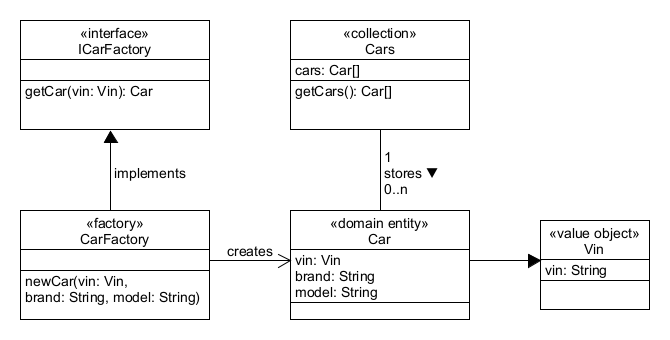
\includegraphics[width=0.8\textwidth]{figures/microservices/dmCar/apiDiagramDM-CarExtended.png}
    \caption{Alternative API Diagram of DM-CarV1.0}
    \label{fig:api_diagram_dm_car_alternative}
\end{figure}

\subsection{Excercise PrepareLocalWorkingFolder}
\label{subsec:prepare_local_working_folder}